\begin{figure*}[t]
\checkoddpage \ifoddpage \forcerectofloat \else \forceversofloat \fi
\frame{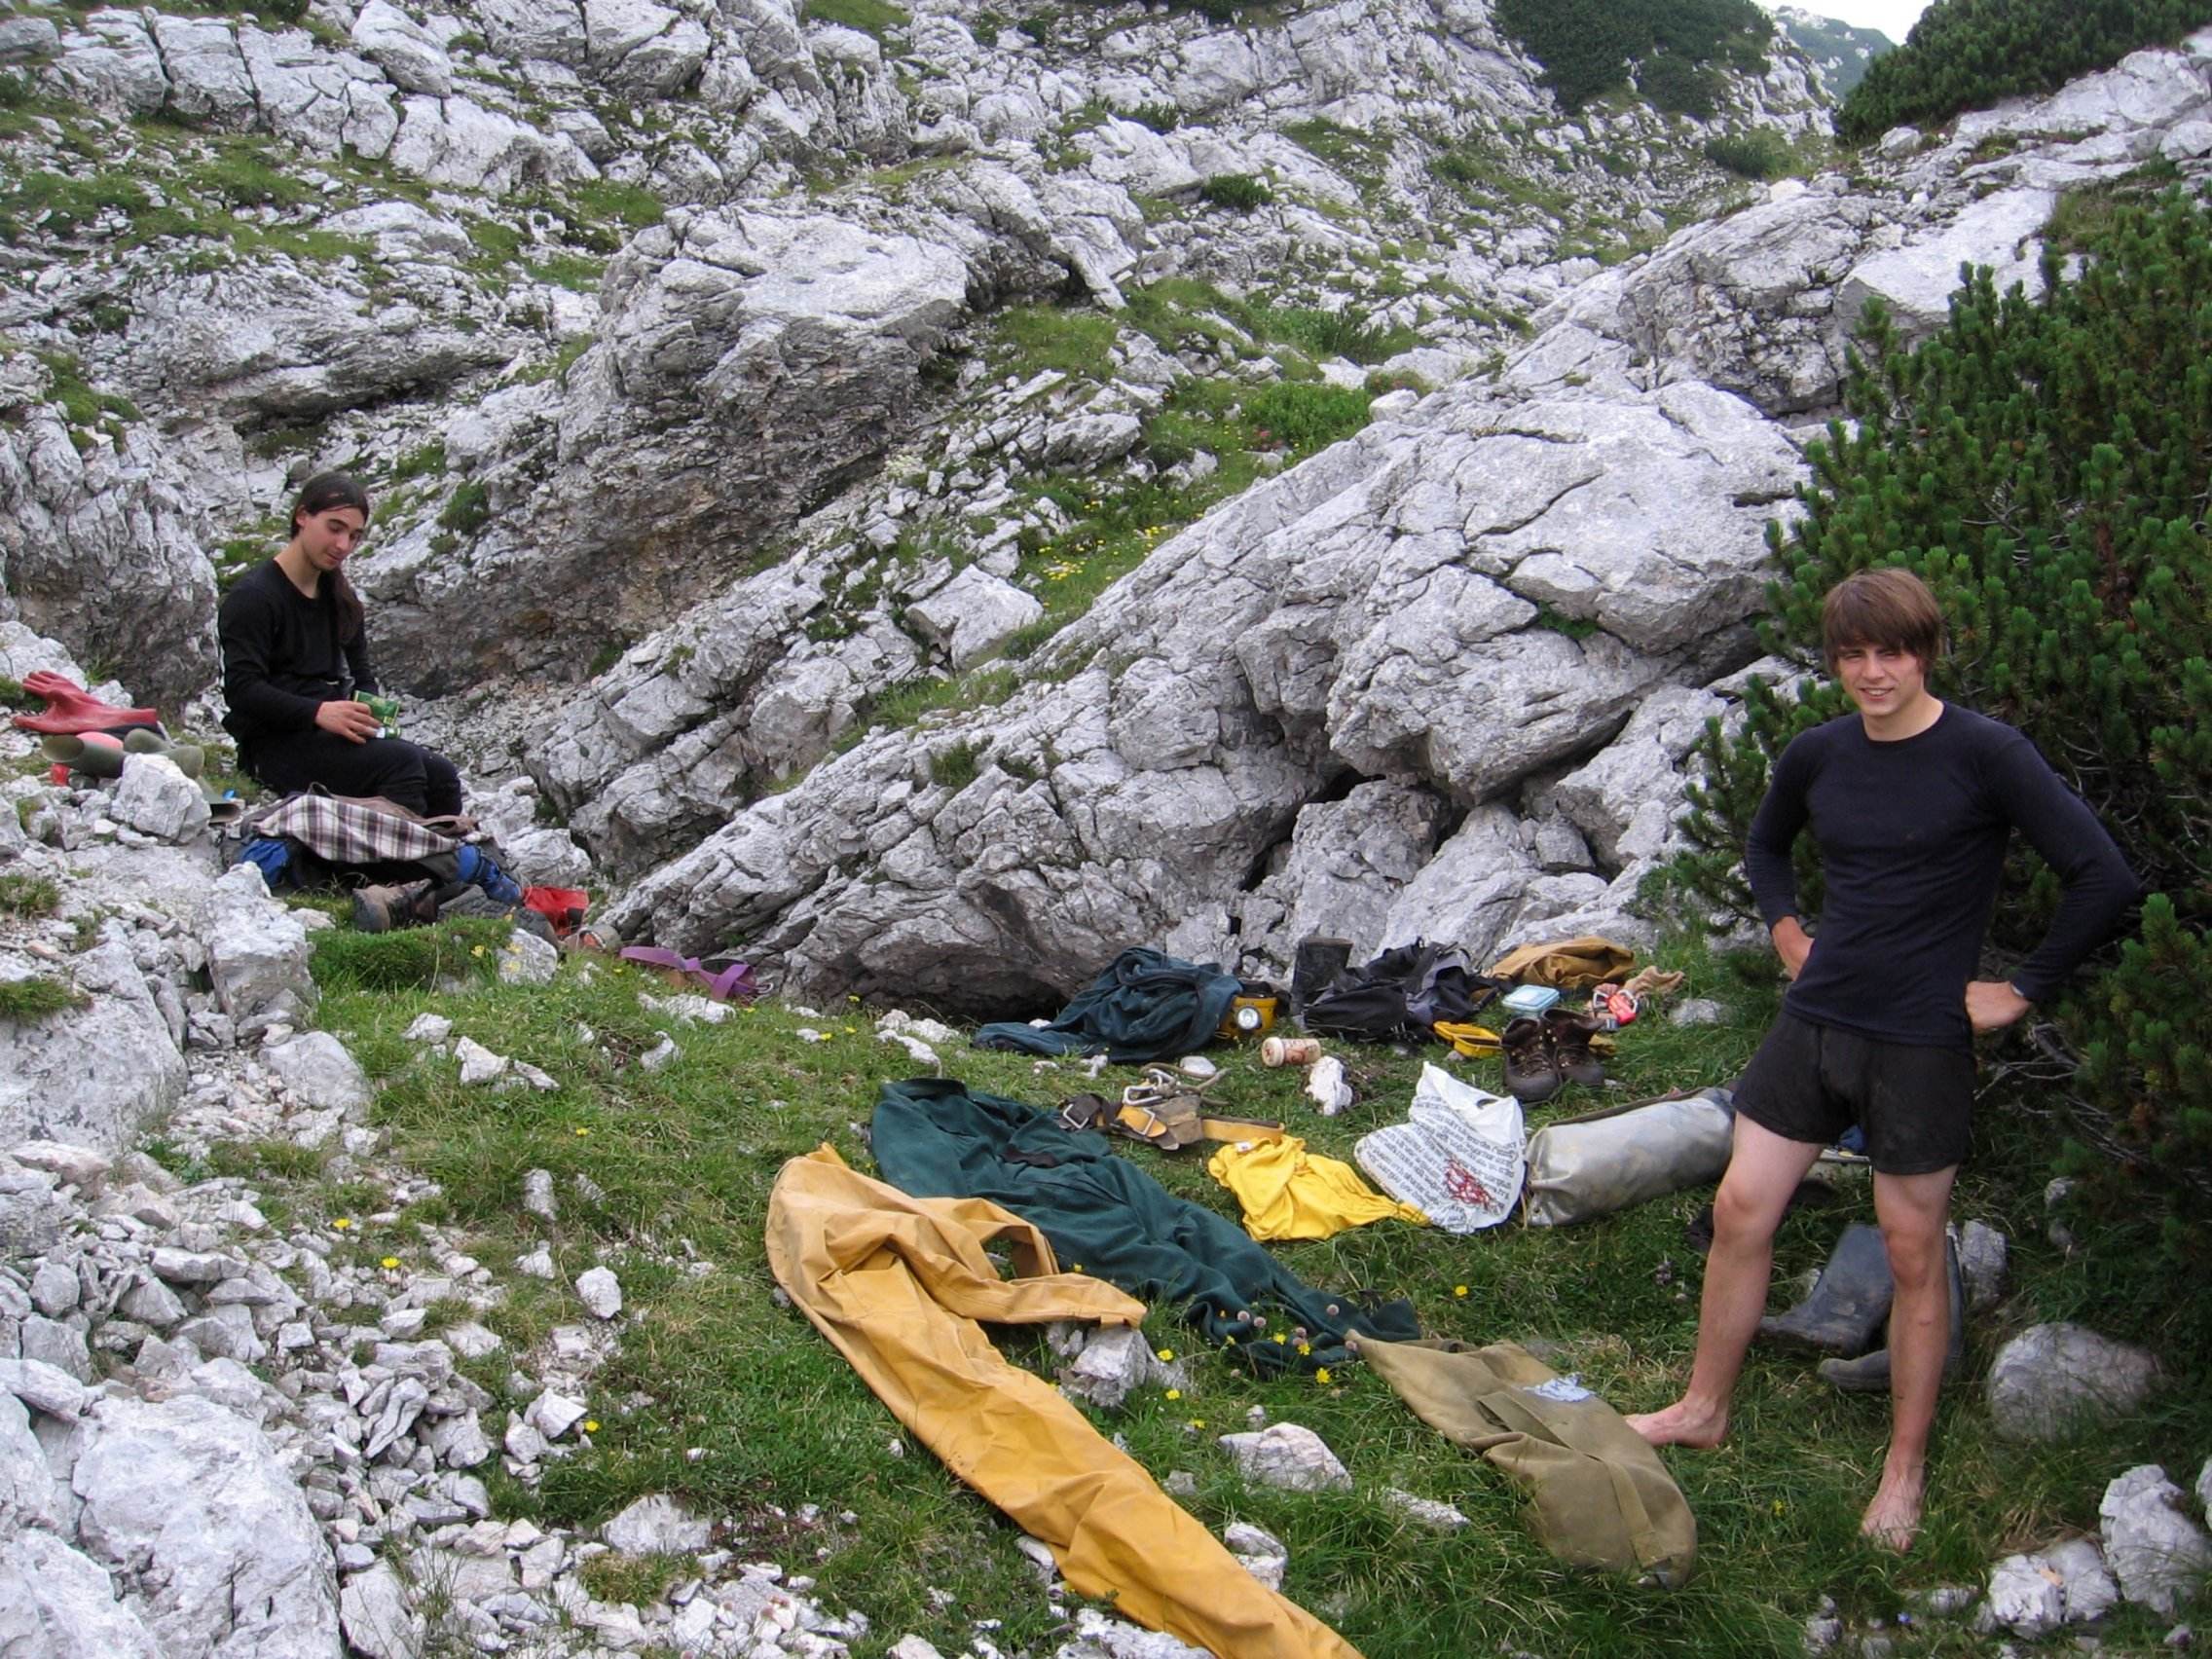
\includegraphics[width=\linewidth]{2008/vilinska/Jarvist Frost - canon a520 - gw - ck team getting ready at entrance to gw--orig.jpg}}
\caption{Izi and Paul changing outside the entrance of \protect\passage{Gardeners' World}. \protect\passage{Vilinska Jama} was connected to \protect\passage{Gardeners' World}, becoming the second entrance to the larger cave. \pic{Jarvist Frost}}
\end{figure*}

\section{Tetley's mysterious lead}

Tetley led the way down past \passage{Gardeners' World}, only grudgingly agreeing that blindfolds would not be required. The entrance is an unwelcoming yet
strangely inviting scree slope under a bedding plane, with a howling and
glacial draft emerging from it.

We headed down, leaving Janet at the surface to see off any would-be
unsurpers of the joys within. The way on quickly opens up to a chamber
with a snow plug then regresses just as quickly to a tight, boulder
filled, rift. Tetley started chiselling away at a constriction. Dan took
over while Tetley dug underneath, bypassing the squeeze entriely. More
up and down around the boulders led to an impassably tight pitch head.
Tetley and Dan made slow progress with chisels until Bozo arrived, having
extracted our location from Janet. A few mighty blows later, the way on
was clear (still tight though - will need more destruction).

\tweet{6:16PM Jul 31, 2008}{GW now system with con of VILINSKA to bot of laurel.Kangaroo going strong,P45 DARK TRANQUILITY on 15hr 4man trip.M2 pushed >70s camp.}

Tetley rigged a ladder from a securely wedged boulder, and Dan clambered
down into a boulder strewn chamber. Water was dripping from a crack in
the ceiling, and the rift continued ahead. 

``Does it go?'' shouted
Tetley. 

``Game on!'' came the reply.

Bozo forged ahead, quickly finding another chamber, filled with a vast
two way boulder slope. Up and over choked quickly. Down and under was
precarious in the extreme, but Tetley's careful progress under the
hanging death and down a short climb yielded the next pitch. A
$\approx$ 20 m drop into a large fault controlled chamber. With no
SRT kit or rope we made our exit, pausing briefly to discuss potential
names. We settled on \passage{Vilinska Jama} (Veela cave) and returned to the \passage{Bivi}
for Tea \& Medals. 

\name{Dan Greenwald}

\begin{figure*}[t!]
      \checkoddpage \ifoddpage \forcerectofloat \else \forceversofloat \fi
      \centering
    \begin{subfigure}[t]{\textwidth}
    \centering
        \frame{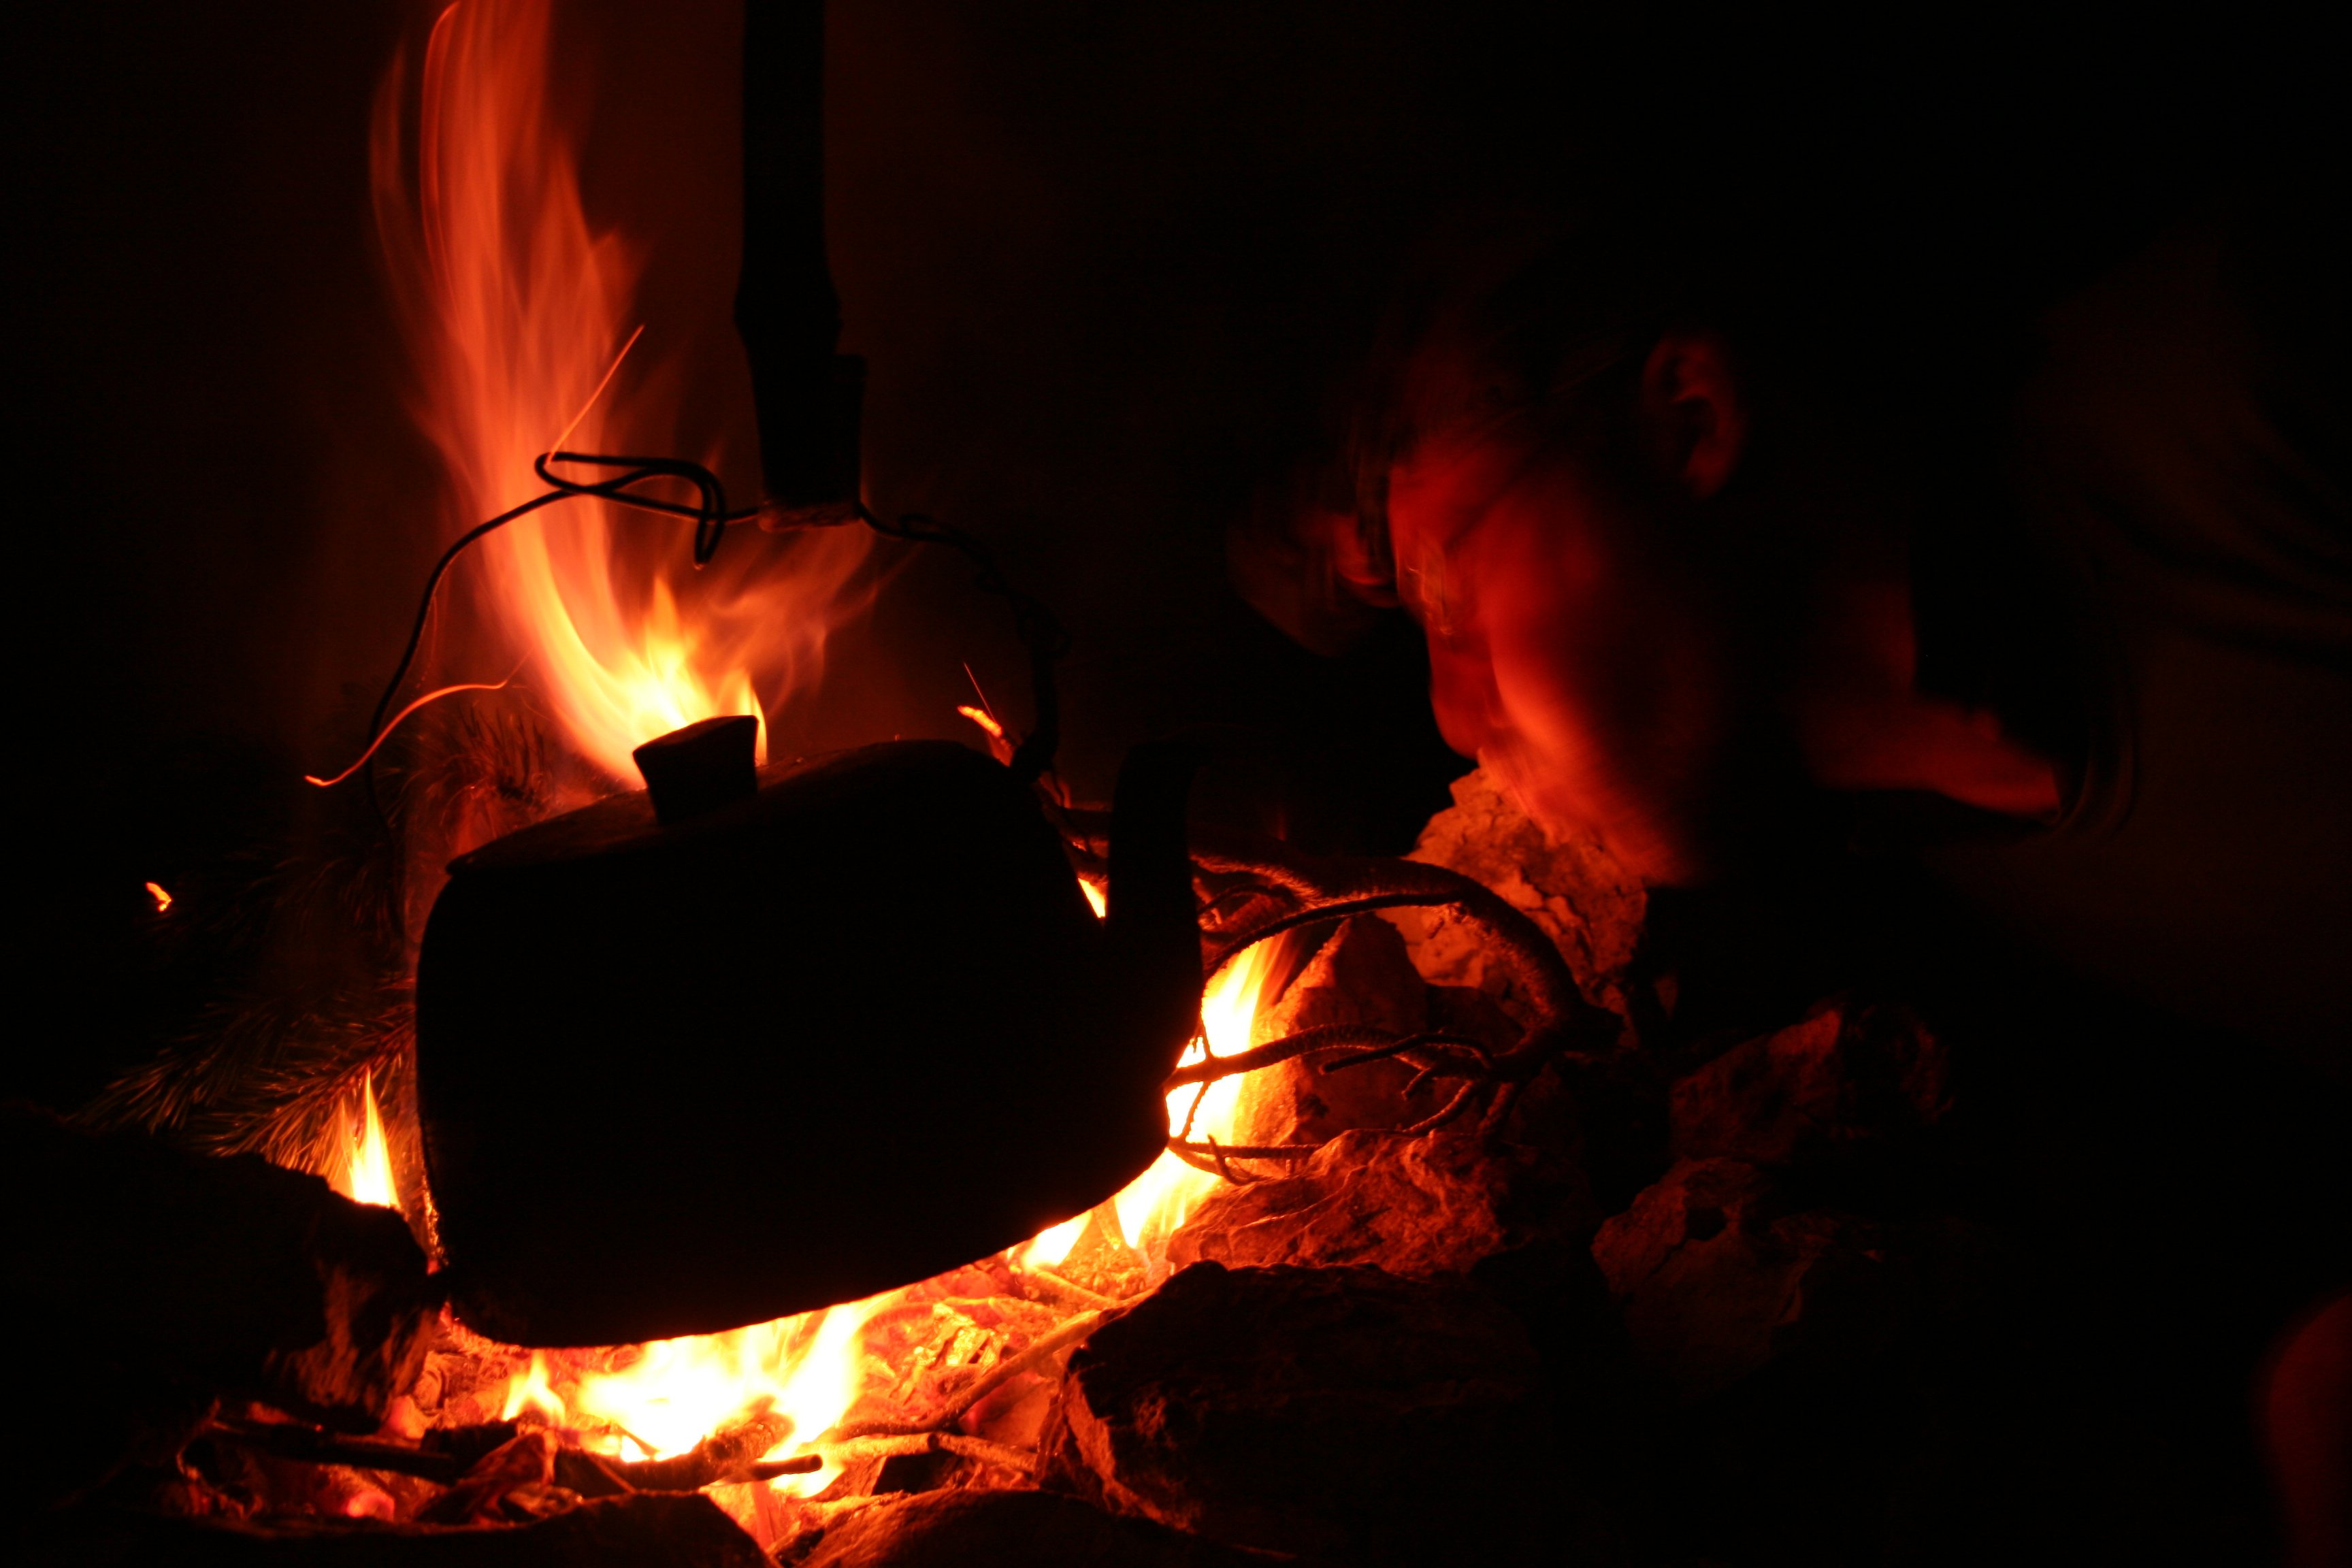
\includegraphics[width=\linewidth]{2008/vilinska/Jana Carga - Canon 350D - img_3115 tetley blowing the fire to brew tea--orig.jpg}} 
        \caption{} \label{tea bivi}
    \end{subfigure}
    
          \vspace{0.3cm}
          
    \begin{subfigure}[t]{0.49\textwidth}
        \centering
        \frame{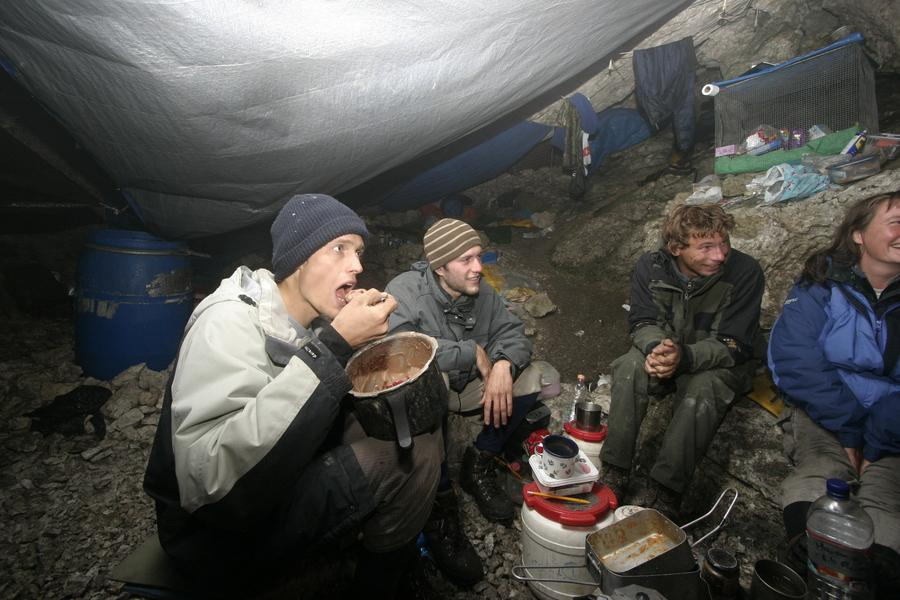
\includegraphics[width=\linewidth]{2008/vilinska/MMslov08 58--orig.jpg}} 
        \caption{} \label{jarvist anal}
    \end{subfigure}
    \hfill
    \begin{subfigure}[t]{0.49\textwidth}
        \centering
        \frame{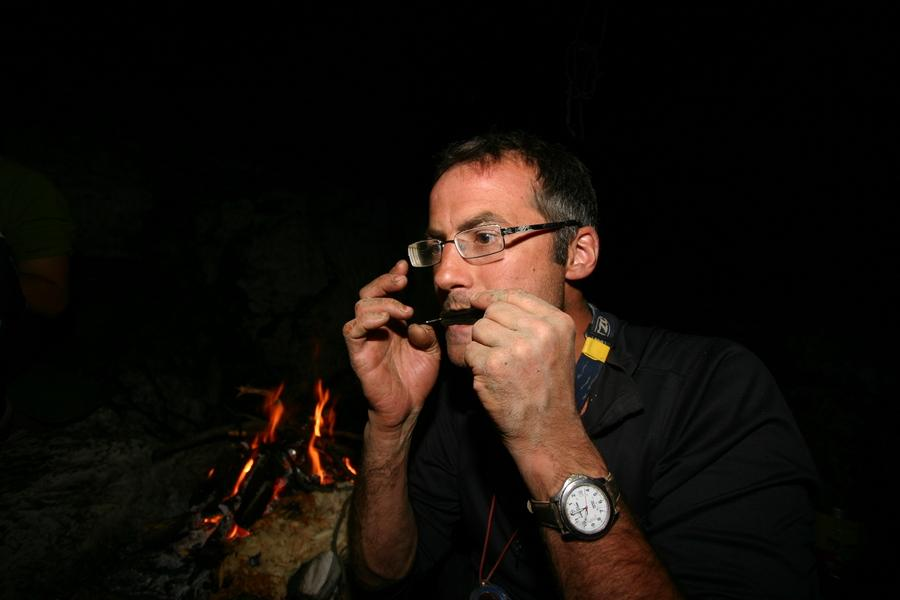
\includegraphics[width=\linewidth]{2008/vilinska/MMslov08 29--orig.jpg}} 
        \caption{} \label{tetley jawharp}
    \end{subfigure}

    \caption{\passage{Bivi} nights.
    \textit{(a)} The teapot in the \passage{Bivi} fire. \pic{Jarvist Frost}   \textit{(b)} Angel delight, which is made (and eaten) communally by handing around the pan and a whisk and beating the mixture until you tire and pass it on, is a popular evening pudding.
    \textit{(c)} Tetley's musical instrument of choice in 2008 was the jawharp. \pic{Martin McGowan}}
\end{figure*}